% ============================================================
% Lecture 9 -- Theory of linear models
% ============================================================
\section{Theory of Linear Models}\label{sec:L09}

\lectureheader{9}{kAKqc2ftwaA}{Week-3 handwritten notes \texttt{Feb9.pdf}, part ``Theory of linear models'' (definition, remark, examples, matrix notation)}

\begin{guiding*}
By the end of this lecture you should be able to:
\begin{itemize}
  \item state the general definition of a linear model and explain why it is called \emph{linear};
  \item write the one-way, nested and two-way classification models in this form;
  \item express any linear model in matrix notation as $(Y,X\beta,\sigma^2I_n)$ and compute $\EE[Y]$ and $\Cov(Y)$.
\end{itemize}
\end{guiding*}

\subsection{Recap}
\Cref{sec:L08} studied one particular model, the one-way classification, and wrote it as
$Y=X\beta+\eps$. We now define the general class of models of this kind.

\subsection{Definition}
\begin{definition}[Linear model]\label{def:L09-linmodel}
Suppose we have $n$ observations $\{y_1,\dots,y_n\}$ that are realisations of random variables
$Y_1,\dots,Y_n$. Let $(\beta_1,\dots,\beta_p)$ be the parameters on which the distribution of the
data depends. A \vocab{linear model} is
\[
Y_i=x_{i1}\beta_1+x_{i2}\beta_2+\dots+x_{ip}\beta_p+\eps_i,\qquad 1\le i\le n,
\]
where $\eps_1,\dots,\eps_n$ are \emph{uncorrelated} random variables with $\EE(\eps_i)=0$ and
$\Var(\eps_i)=\sigma^2$ for $1\le i\le n$, and the $x_{ij}$ are known constants.
\end{definition}
(The instructor writes $m$ for the number of parameters. We use $p$; see the notation table.)

\begin{remark}\label{rem:L09-alt}
The model can equivalently be described by
\[
\EE[Y_i]=\sum_{j=1}^p x_{ij}\beta_j\quad(1\le i\le n),\qquad
Y_1,\dots,Y_n \text{ uncorrelated with } \Var(Y_i)=\sigma^2 .
\]
It is called \emph{linear} because the expected value is linear \emph{in the parameters}
$\beta_1,\dots,\beta_p$. It need not be linear in the explanatory variables.
\end{remark}

\begin{note}
Normality is \emph{not} part of the definition. Only means, variances and uncorrelatedness are
assumed. Everything about least squares and the Gauss--Markov theorem needs only these second-order
assumptions. Normality is added later (Week~6, ``Assumption of normality'') to obtain exact
distributions for tests and confidence intervals, as we already did in \cref{thm:L08-dist}.
\end{note}

\begin{example}[Linear in $\beta$, not in $x$]\label{ex:L09-poly}
The quadratic regression $Y_i=\beta_1+\beta_2t_i+\beta_3t_i^2+\eps_i$ is a linear model, with
$x_{i1}=1$, $x_{i2}=t_i$, $x_{i3}=t_i^2$. So is $Y_i=\beta_1+\beta_2\log t_i+\eps_i$. The model
$Y_i=\beta_1e^{\beta_2t_i}+\eps_i$ is \emph{not} linear, because $\beta_2$ enters non-linearly.
\end{example}

\subsection{Examples: classification models}
\begin{example}[One-way classification]\label{ex:L09-oneway}
$Y_{ij}=\mu+\mu_i+\eps_{ij}$, $1\le i\le k$, $1\le j\le n_i$ (\cref{def:L08-oneway}). The
parameters are $(\mu,\mu_1,\dots,\mu_k)$. For observation $(i,j)$ the coefficient of $\mu$ is $1$,
the coefficient of $\mu_i$ is $1$, and all others are $0$.
\end{example}

\begin{example}[Nested classification]\label{ex:L09-nested}
\[
Y_{ijl}=\mu+\mu_i+\delta_{ij}+\eps_{ijl},\qquad 1\le l\le n_{ij},\ 1\le j\le m_i,\ 1\le i\le k .
\]
There are $k$ groups. Group $i$ contains $m_i$ subgroups, and $n_{ij}$ observations are taken in
subgroup $j$ of group $i$. For example, $k$ schools, $m_i$ classes in school $i$, and $n_{ij}$
pupils in class $j$. $\delta_{ij}$ is the effect of subgroup $j$ \emph{within} group $i$. The
subgroups are nested: class 1 of school 1 has nothing to do with class 1 of school 2. The
parameter vector has $1+k+\sum_i m_i$ entries.
\end{example}

\begin{example}[Two-way classification with interaction]\label{ex:L09-twoway}
\[
Y_{ijl}=\mu+\alpha_i+\beta_j+\gamma_{ij}+\eps_{ijl},\qquad 1\le l\le n_{ij},\ 1\le j\le J,\ 1\le i\le I .
\]
Two factors cross each other: factor $A$ with $I$ levels (effects $\alpha_i$) and factor $B$ with
$J$ levels (effects $\beta_j$). $\gamma_{ij}$ is the \emph{interaction}, the extra effect of the
combination $(i,j)$. The notes label this model ``three way classification''. It is the model
the Week-5 assignment calls the two-way classification. There are $1+I+J+IJ$ parameters.
\end{example}

\subsection{Matrix notation}
\begin{definition}[Matrix form]\label{def:L09-matrix}
Put
\[
Y=(Y_1,\dots,Y_n)\T,\quad \beta=(\beta_1,\dots,\beta_p)\T,\quad X=(x_{ij})_{1\le i\le n,\,1\le j\le p},\quad \eps=(\eps_1,\dots,\eps_n)\T .
\]
Then the linear model reads
\[
\underset{n\times1}{Y}=\underset{n\times p}{X}\;\underset{p\times1}{\beta}+\underset{n\times1}{\eps},
\qquad \EE[\eps]=0,\quad \Cov(\eps)=\sigma^2I_n .
\]
We denote it by $(Y,X\beta,\sigma^2I_n)$. The three entries are the observations, their
expectation $\EE[Y]=X\beta$, and the variance--covariance matrix of the data.
\end{definition}

To work with $\Cov$ we recall its definition and the two rules used constantly from now on.
\begin{definition}[Mean vector and covariance matrix]\label{def:L09-cov}
For a random vector $W\in\RR^n$, $\EE[W]=(\EE W_1,\dots,\EE W_n)\T$ and
$\Cov(W)=\EE\bigl[(W-\EE W)(W-\EE W)\T\bigr]$, the $n\times n$ matrix with entries $\Cov(W_i,W_l)$.
\end{definition}

\begin{proposition}\label{prop:L09-rules}
For a random vector $W\in\RR^n$, a fixed $q\times n$ matrix $A$ and a fixed $b\in\RR^q$:
\[
\EE[AW+b]=A\,\EE[W]+b,\qquad \Cov(AW+b)=A\Cov(W)A\T .
\]
In particular, in the linear model $\EE[Y]=X\beta$ and $\Cov(Y)=\sigma^2I_n$.
For a fixed vector $\ell\in\RR^n$, $\EE[\ell\T Y]=\ell\T X\beta$ and $\Var(\ell\T Y)=\sigma^2\pnorm{\ell}^2$.
\end{proposition}
\begin{proof}
The $r$th entry of $AW+b$ is $\sum_l a_{rl}W_l+b_r$. Its expectation is $\sum_l a_{rl}\EE W_l+b_r$
by linearity of expectation, which is the $r$th entry of $A\EE W+b$. Next,
$AW+b-\EE[AW+b]=A(W-\EE W)$, so
\[
\Cov(AW+b)=\EE\bigl[A(W-\EE W)(W-\EE W)\T A\T\bigr]=A\,\EE\bigl[(W-\EE W)(W-\EE W)\T\bigr]A\T=A\Cov(W)A\T ,
\]
again by linearity (entry by entry). For the linear model take $W=\eps$, $A=I$, $b=X\beta$. Then
$Y=\eps+X\beta$ gives $\EE Y=X\beta$ and $\Cov(Y)=\Cov(\eps)=\sigma^2I$. Finally take $A=\ell\T$ ($q=1$):
$\Var(\ell\T Y)=\ell\T(\sigma^2I)\ell=\sigma^2\pnorm{\ell}^2$.
\end{proof}

\begin{example}[Matrix form of simple linear regression]\label{ex:L09-slr}
$Y_i=\beta_1+\beta_2x_i+\eps_i$, $i=1,\dots,4$, with $x=(1,2,3,4)$:
\[
Y=\begin{pmatrix}Y_1\\Y_2\\Y_3\\Y_4\end{pmatrix},\quad
X=\begin{pmatrix}1&1\\1&2\\1&3\\1&4\end{pmatrix},\quad
\beta=\begin{pmatrix}\beta_1\\\beta_2\end{pmatrix},\quad
\EE[Y]=\begin{pmatrix}\beta_1+\beta_2\\\beta_1+2\beta_2\\\beta_1+3\beta_2\\\beta_1+4\beta_2\end{pmatrix},\quad
\Cov(Y)=\sigma^2I_4 .
\]
Here $n=4$, $p=2$ and $\rank(X)=2$. The two columns are not proportional.
\end{example}

\begin{example}[Matrix form of a small nested model]\label{ex:L09-nested-mat}
Take $k=2$ groups, each with $m_i=2$ subgroups and $n_{ij}=1$ observation. With
$\beta=(\mu,\mu_1,\mu_2,\delta_{11},\delta_{12},\delta_{21},\delta_{22})\T$ and
$Y=(Y_{111},Y_{121},Y_{211},Y_{221})\T$:
\[
X=\begin{pmatrix}
1&1&0&1&0&0&0\\
1&1&0&0&1&0&0\\
1&0&1&0&0&1&0\\
1&0&1&0&0&0&1
\end{pmatrix}.
\]
Here $n=4$, $p=7$ and $\rank(X)=4$: the last four columns form $I_4$. There are many more
parameters than identifiable combinations. \Cref{sec:L11} writes out larger examples.
\end{example}

\begin{figure}[ht]
\centering
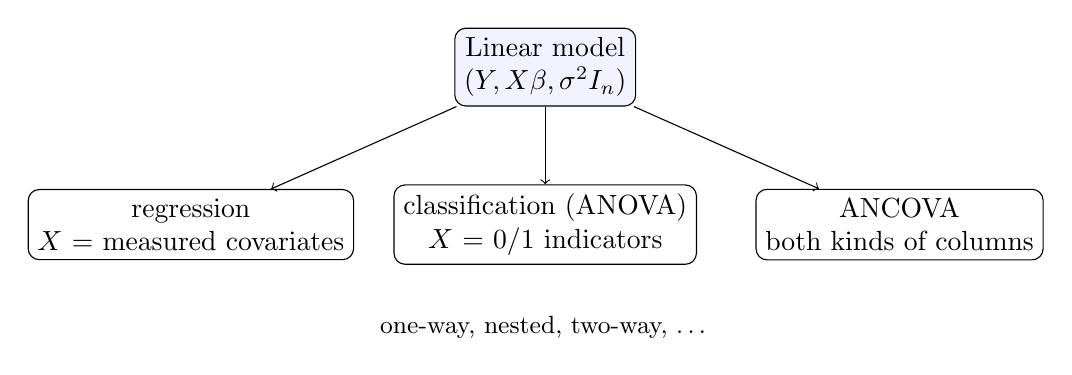
\begin{tikzpicture}[scale=1.0]
\node[draw,rounded corners,fill=blue!5,align=center] (lm) at (0,0) {Linear model\\$(Y,X\beta,\sigma^2I_n)$};
\node[draw,rounded corners,align=center] (reg) at (-4.5,-2) {regression\\$X$ = measured covariates};
\node[draw,rounded corners,align=center] (cls) at (0,-2) {classification (ANOVA)\\$X$ = 0/1 indicators};
\node[draw,rounded corners,align=center] (anc) at (4.5,-2) {ANCOVA\\both kinds of columns};
\draw[->] (lm) -- (reg); \draw[->] (lm) -- (cls); \draw[->] (lm) -- (anc);
\node[font=\small,align=center] at (0,-3.3) {one-way, nested, two-way, \dots};
\end{tikzpicture}
\caption{All models in this course are special cases of $(Y,X\beta,\sigma^2I_n)$. They differ only in the design matrix.}
\label{fig:L09-family}
\end{figure}

\subsection{Computation}
The notebook \nb{week03/L09\_theory\_linear\_models.ipynb} builds the design matrices of
\cref{ex:L09-slr,ex:L09-nested-mat} and of a two-way model with \texttt{numpy}, and also with
\texttt{patsy}/\texttt{statsmodels} formulas. It computes their ranks and checks
$\Cov(AY)=A\Cov(Y)A\T$ by simulation.

\subsection{Summary}
\begin{itemize}
  \item Linear model: $Y_i=\sum_j x_{ij}\beta_j+\eps_i$, with $\eps_i$ uncorrelated, $\EE\eps_i=0$, $\Var\eps_i=\sigma^2$. It is linear in the \emph{parameters}.
  \item Matrix form $(Y,X\beta,\sigma^2I_n)$: $Y=X\beta+\eps$, $\EE Y=X\beta$, $\Cov Y=\sigma^2I_n$.
  \item $\EE[AW+b]=A\EE W+b$ and $\Cov(AW+b)=A\Cov(W)A\T$. In particular $\Var(\ell\T Y)=\sigma^2\pnorm{\ell}^2$.
  \item Classification models (one-way, nested, two-way) are linear models with 0/1 design matrices.
\end{itemize}

\subsection{Exercises}
\begin{problem}\label{prob:L09-1}
Write the design matrix of the two-way model with interaction for $I=J=2$ and $n_{ij}=1$. What is its rank?
\end{problem}
\begin{problem}\label{prob:L09-2}
Which of the following are linear models? (a) $Y_i=\beta_1+\beta_2\sin t_i+\eps_i$; (b) $Y_i=\beta_1t_i^{\beta_2}+\eps_i$; (c) $Y_i=(\beta_1+\beta_2)t_i+\eps_i$.
\end{problem}
\begin{problem}\label{prob:L09-3}
In the linear model, find $\Cov(\bar Y,Y_1-\bar Y)$ where $\bar Y=\frac1n\sum Y_i$.
\end{problem}
\begin{problem}\label{prob:L09-4}
Let $W$ be a random vector with $\Cov(W)=\Sigma$. Show that $\Sigma$ is symmetric and positive semi-definite.
\end{problem}

\subsection{Further reading}
Christensen, \S1.1 (random vectors and matrices) and the introduction to Chapter~2. Rao, \S1b
(matrices) and \S4a.1 (the Gauss--Markoff set-up). Weisberg, \emph{ALR}, Chapter~3.
